\section{The notch and its dominated region}
\label{sec:model}

The behavioural response to the registration notch is documented in
administrative data by \citet{liuetal2021}; the synthetic data contain no
bunching signal to exploit (Section~\ref{sec:bunching}). To characterise the
notch precisely I therefore turn to its analytic structure, which yields an
exact distortion measure that needs no behavioural calibration. I set out the
firm-level structure following \citet{klevenwaseem2013}, \citet{saez2010}, and
\citet{kleven2016}, whose bunching framework \citet{liuetal2021} adapt to UK
VAT. The UK registration threshold is a \emph{notch}, not a kink: once
turnover crosses the threshold the firm becomes liable for VAT on its
\emph{entire} base, not merely on the increment above it. The section's
central deliverable is the notch's \emph{dominated region}---an exact,
elasticity-free property of the schedule that indexes the distortion the
threshold imposes (Section~\ref{ssec:dominated})---and its analytic response
to each schedule reform, complementing the static reform costs of
Section~\ref{ssec:schedule_costs}. Section~\ref{sec:behavioural} prices the
intensive-margin response to each reform conditional on an assumed turnover
elasticity; nothing in this section depends on that assumption.

\paragraph{Scope.} The model prices the registration margin for firms that
remit positive net VAT. Two populations are outside its scope and are treated
as such throughout: below-threshold \emph{voluntary} registrants (roughly 43\%
of eligible firms in \citealp{liuetal2021}), who have chosen registration and
so face no notch at the threshold, and net-repayment traders (zero-rated
exporters and similar), whose remittance is negative for rated-structure
reasons the generator does not represent (Section~\ref{sec:data}).

\subsection{The firm's problem}

Each firm $i$ chooses turnover $y_i$ to maximise after-tax profit. Let $c_i(y_i)$
denote the cost of producing turnover $y_i$, $T^{*}$ the registration threshold,
and $\tau$ the standard VAT rate. In the simplest statement VAT applies to the
firm's entire turnover once it registers, so after-tax revenue is discontinuous
and profit is
\begin{equation}
  \pi_i(y_i) \;=\;
  \begin{cases}
    \;y_i - c_i(y_i), & y_i < T^{*} \quad \text{(unregistered)},\\[4pt]
    \;(1-\tau)\,y_i - c_i(y_i), & y_i \ge T^{*} \quad \text{(registered)}.
  \end{cases}
  \label{eq:firm-problem}
\end{equation}
At $T^{*}$ after-tax revenue falls discretely by $\tau\,T^{*}$: a firm
that nudges its turnover from just below to just above the threshold loses
$\tau\,T^{*}$ of net revenue on turnover it was already earning. With the
standard rate $\tau=0.20$ and threshold $T^{*}=\pounds85{,}000$ this discrete
drop is $\tau\,T^{*}=\pounds17{,}000$ on whole turnover. Real VAT taxes value
added, and the corrected data give each firm net liability
$v_i=\tau(y_i-x_i)$ with deductible inputs $x_i=\delta_i y_i$
(Section~\ref{sec:data}); profit is then
$(1-\delta_i)y_i - \tilde c_i(y_i)$ unregistered and
$(1-\delta_i)(1-\tau)y_i - \tilde c_i(y_i)$ registered---the deductible share
multiplies \emph{both} branches, so the notch geometry
of~\eqref{eq:firm-problem} carries over firm by firm, with the cash size of
the jump scaled to $\tau(1-\delta_i)T^{*}$ (about \pounds6{,}800 at the mean
value-added share of 40\%). This drop---absent from a kink, where only the
\emph{marginal} rate changes at the threshold while average liability moves
continuously---is the defining feature of a notch: it makes locating just
below the cutoff strictly attractive and creates the empty band derived next.
Throughout, the firm is assumed to bear the full statutory rate on its value
added---no pass-through to prices---so the notch geometry is stated in terms
of the firm's own net revenue; with partial pass-through the cash size of the
jump, and the width derived next, would shrink in proportion to the share
borne by the firm.

\subsection{The dominated region}
\label{ssec:dominated}

The notch creates a range of turnover just above $T^{*}$ that no
profit-maximising firm chooses under the model. A firm just below the threshold
earns net revenue $T^{*}$; a registered firm at $T^{*}+a$ earns
$(1-\tau)(T^{*}+a)$. Before these net revenues become equal, the registered
firm receives less net revenue while producing more. Thus, for any
non-decreasing production cost, it earns strictly lower profit; no locally
constant-cost approximation is required. Equating net revenues defines the
boundary of this guaranteed dominated region:
\begin{equation}
  (1-\tau)\,(T^{*}+a) \;=\; T^{*}
  \quad\Longrightarrow\quad
  a \;=\; T^{*}\,\frac{\tau}{1-\tau} .
  \label{eq:dominated}
\end{equation}
This is the Kleven--Waseem guaranteed dominated-region width
\citep{klevenwaseem2013}. At
my parameters it gives $a = \pounds85{,}000\times 0.20/0.80 = \pounds21{,}250$,
so the dominated region is
$(T^{*},\,T^{*}+a)=(\pounds85{,}000,\ \pounds106{,}250)$, shown in
Figure~\ref{fig:notch_fit}.

Two properties make this band a transparent index of the distortion. First, it
is \emph{exact and elasticity-free}, and---less obviously---\emph{invariant to
the firm's input share}. Under the value-added formulation above, the
indifference condition at the edge of the region is
$(1-\delta_i)(T^{*}) = (1-\delta_i)(1-\tau)(T^{*}+a)$: the deductible share
$(1-\delta_i)$ cancels, so every firm with positive value added faces the
\emph{same} dominated width $a=T^{*}\tau/(1-\tau)$, whatever its input
intensity. (A per-firm width built from the net remittance rate, such as
$T^{*}\tau_{0i}/(1-\tau_{0i})$, corresponds to a different technology in which
marginal turnover carries no input cost, and is not used here.) The width
depends on $\tau$ and $T^{*}$ alone---not on the cost specification beyond
monotonicity, any
behavioural elasticity, or any smoothing parameter. Who escapes the notch is a
matter of scope, not of input shares (the invariance is a property of the
formulation: unregistered profit carries the same deductible share, so no
input VAT goes unreclaimed below the threshold; if deregistered firms instead
bore VAT on their inputs, the width would shrink in the input share and
vanish for shares above one half---the input-reclaim margin that drives
voluntary registration, Section~\ref{sec:background}): voluntary registrants escape by choice,
and net-repayment traders have no positive remittance to jump
(the Scope paragraph above). Second, the region is an order of magnitude wider
than the $\sim\pounds1$k region implied by a smoothed \emph{kink}
approximation, and it spans a populous part of the firm distribution: about
124{,}300 weighted in-scope firms in the calibrated synthetic population lie
in the $\pounds85{,}000$--$\pounds106{,}250$ band
(\texttt{results/dominated\_region\_mass.txt}; out-of-scope enterprises face
no notch and are excluded). Because the generator has no location choice, this
counts the firms the data \emph{place} in the band---indexing the size of the
population exposed to the distortion---rather than firms that optimally locate
there; the count is conditional on the log--log within-band fill inside the
coarse ONS bands and on the scope flag (Section~\ref{sec:data}) and would
shift under a different within-band shape. It is the width $a$, not the
count, that is exact.

\paragraph{The region under unreclaimed input VAT.} The invariance above
holds because the value-added formulation lets an unregistered firm deduct
its inputs. In the UK system an unregistered firm cannot reclaim input VAT:
it bears $\tau$ on its standard-rated purchases, which is the mechanism
behind voluntary registration (Section~\ref{sec:background}). With input
share $\delta$ and inputs fully standard-rated, unregistered net revenue is
$y(1-\delta-\tau\delta)$ against $(1-\tau)(1-\delta)y$ registered, and
the indifference condition gives
\begin{equation}
  a(\delta) \;=\; T^{*}\,\frac{\tau\,(1-2\delta)}{(1-\tau)(1-\delta)},
  \qquad a(\delta)=0 \text{ for } \delta\ge\tfrac12 .
  \label{eq:dominated-input}
\end{equation}
The width is firm-specific, falls in the input share, and vanishes once inputs
exceed half of turnover, where registration pays for itself through reclaim.
On the synthetic population the median input share of in-scope firms within
\pounds15{,}000 below to \pounds45{,}000 above the threshold is $0.61$:
only 27.5\% of them face a positive dominated width, the mean width across
all of them is \pounds2{,}070 (\pounds7{,}538 among those with a positive
width), and about $11{,}300$ weighted firms sit inside their own dominated
region, against the $124{,}300$ in the fixed \pounds21{,}250 band
(\texttt{results/dominated\_region\_mass.txt}). The \pounds21{,}250 figure
is therefore the zero-input, zero-pass-through upper bound---the width facing
a firm with no reclaimable inputs. The reform comparisons below do \emph{not}
carry over unchanged: the secondary notch at a reduced-rate band top is a step
between two registered states, so its width $a'$ is $\delta$-invariant, and
for the majority of firms whose primary width is zero a banded reduced rate
\emph{creates} a dominated interval at the band top where none existed,
while a level rise changes nothing for them. The ordering stated below
therefore holds for firms with positive $a(\delta)$; for the rest, the
reduced rate is the only reform among the three that introduces a distortion.
Section~\ref{sec:behavioural} retains the reclaim formulation, in which
higher $\delta$ favours bunching; under $a(\delta)$ the comparative static
reverses, and reconciling the behavioural layer with the input-VAT
formulation is left for future work.

\begin{figure}[htbp]\centering
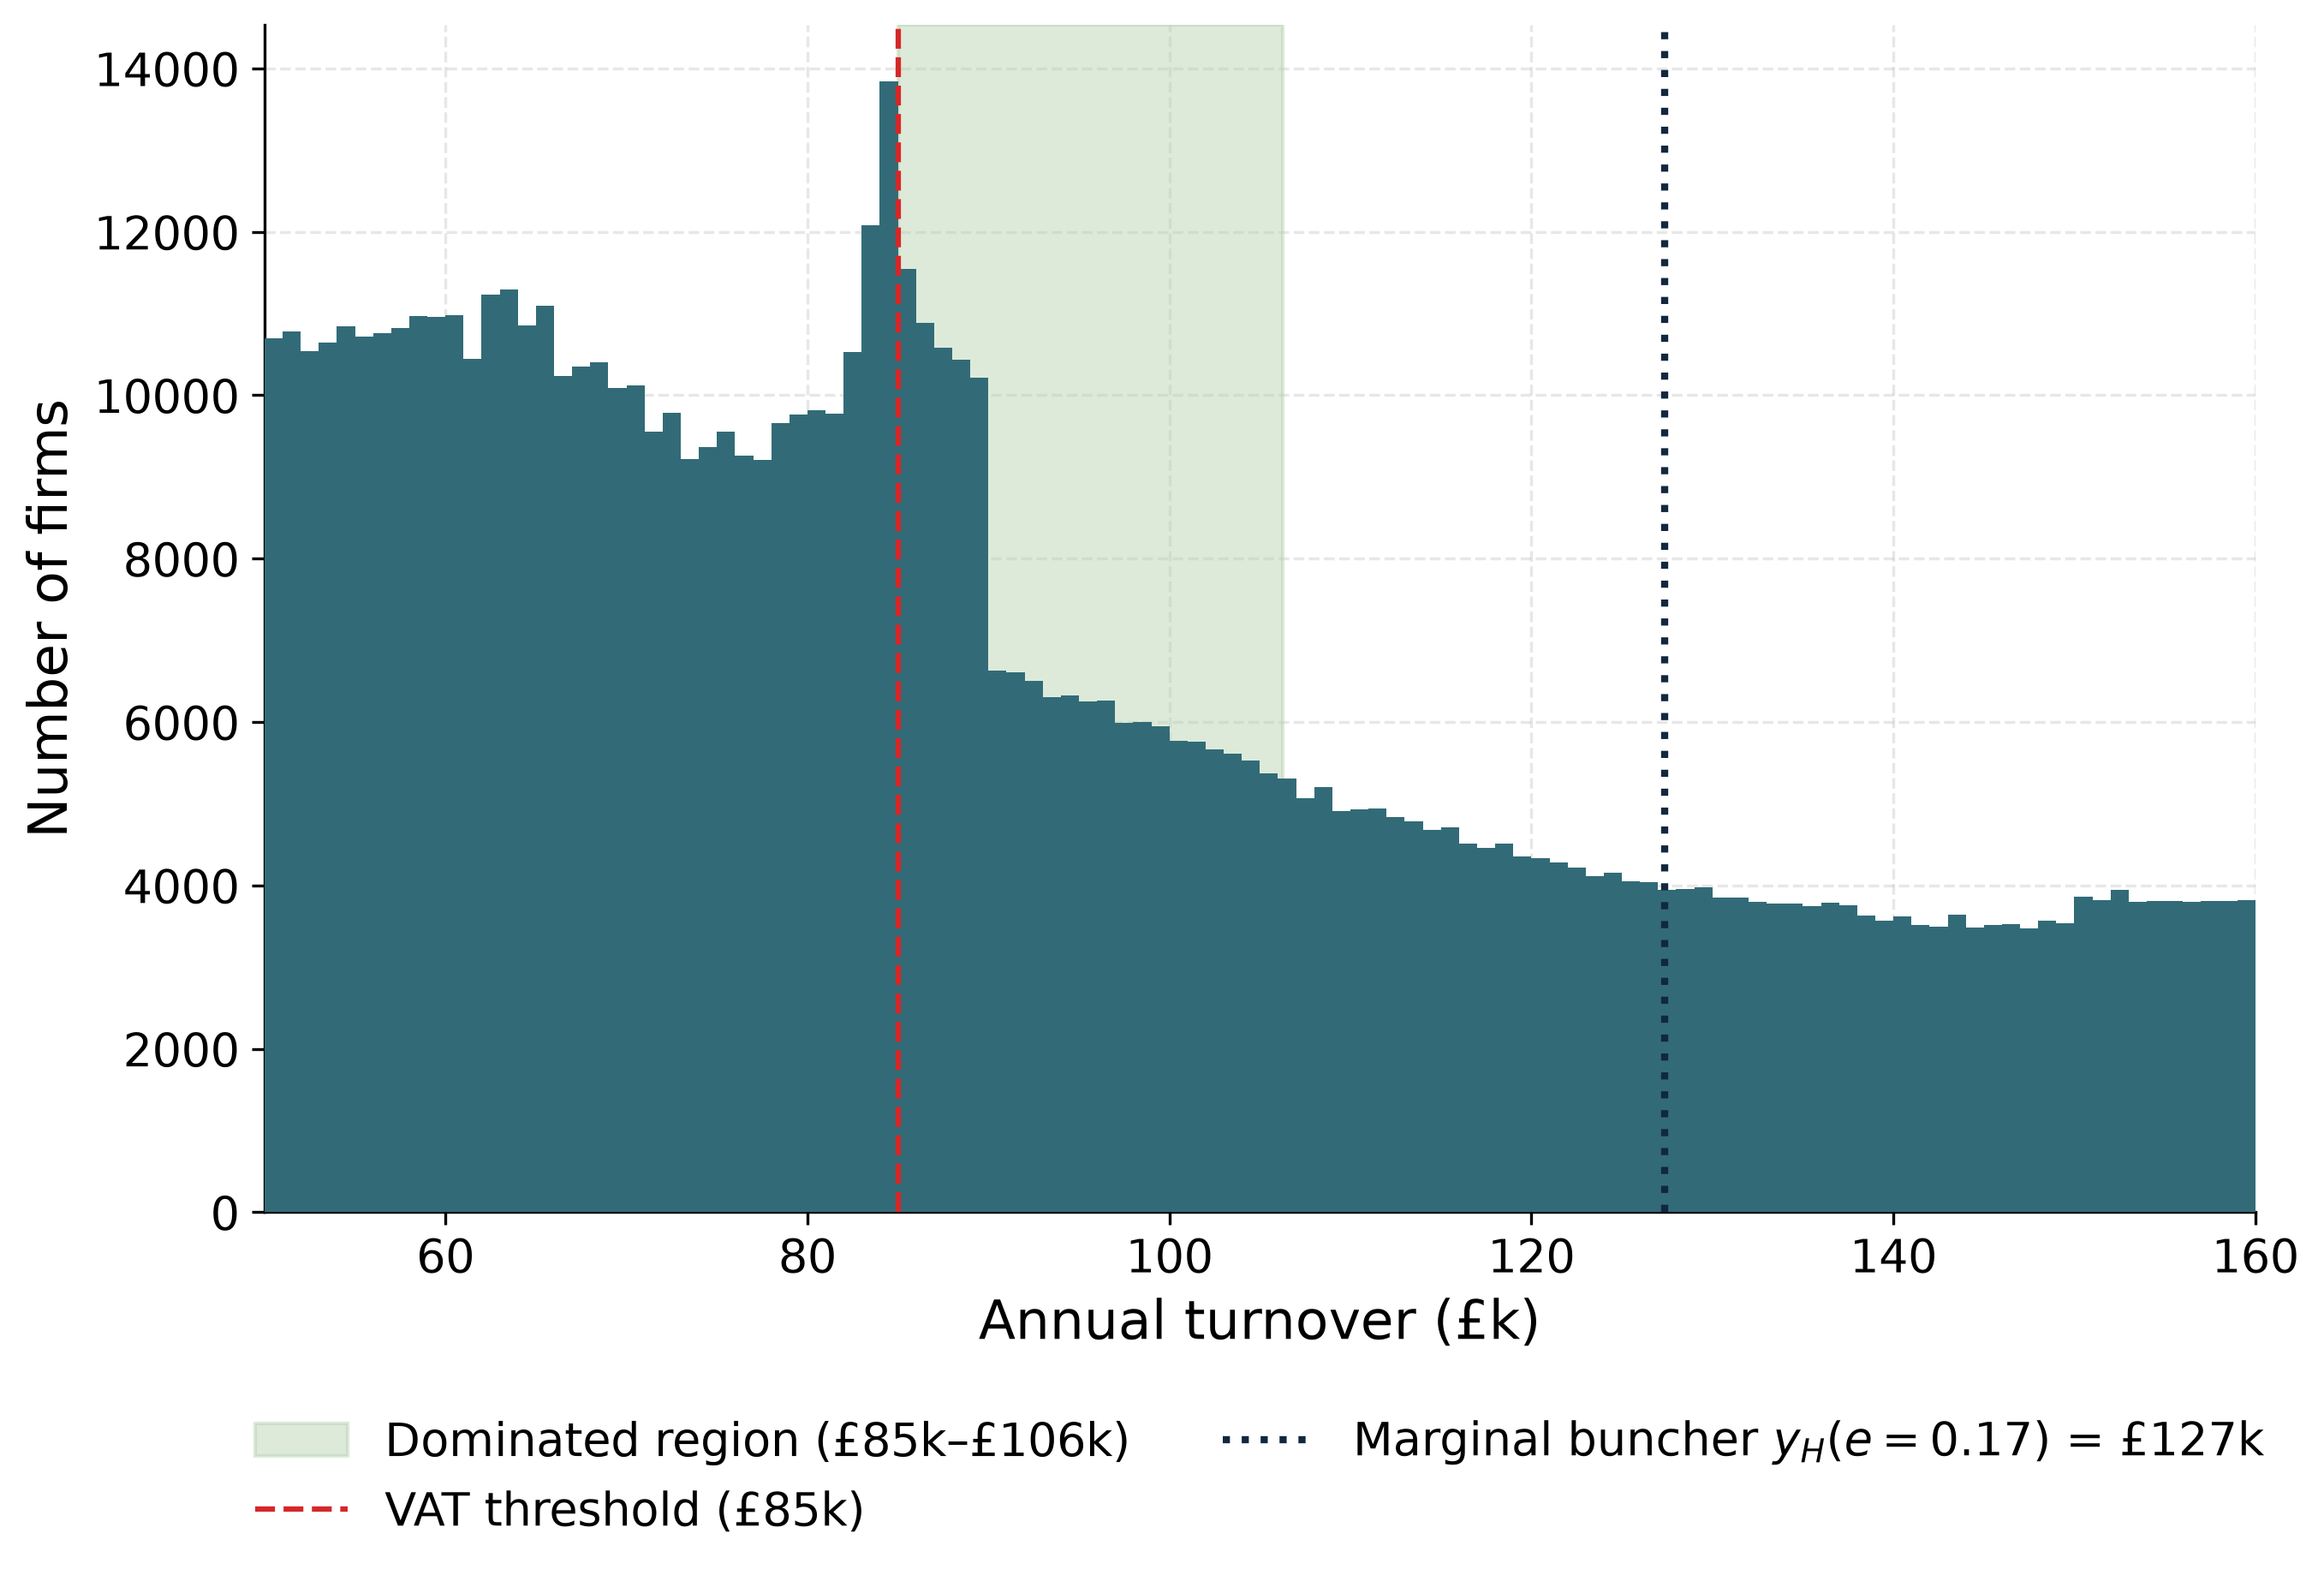
\includegraphics[width=0.96\textwidth]{figures/dynamic_notch_fit_e017.png}
\caption{The VAT notch and the firm distribution. Panel (a) shows net revenue before production costs: immediately above \pounds85{,}000, VAT reduces it from $y$ to $0.8y$, making turnover in $(\pounds85{,}000,\,\pounds106{,}250)$ strictly dominated. Panel (b) shows the three-bin moving mean of weighted 2023--24 in-scope synthetic firm counts, with the same interval shaded. The distribution is descriptive and target-inherited, not the outcome of behavioural optimisation; its drop at \pounds85{,}000 reflects the scope flag---every frame business below the threshold is registrable, while about half of frame enterprises above it are VAT traders---not an empty turnover interval. The vertical lines mark the marginal-buncher \emph{ability} $n_H$ at $e=0.17$ for deductible shares $\delta=0$ and $\delta=0.6$ (Section~\ref{sec:behavioural}); a firm of that ability registers at $n_H[(1-\delta)(1-\tau)]^{e}$, so the lines are not observed-turnover locations. The exact dominated width is $a=\pounds21{,}250$.}
\label{fig:notch_fit}
\end{figure}

\paragraph{How each reform changes the dominated region.} Because the width
$a=T^{*}\tau/(1-\tau)$ depends on the threshold and the rate alone, the effect of
each schedule reform of Section~\ref{ssec:schedule_costs} on the dominated
region is exact and follows directly from the notch arithmetic
of~\eqref{eq:dominated} and~\eqref{eq:dominated-secondary}, with no dependence on
the cost specification beyond monotonicity, any behavioural elasticity, or any simulated
re-optimisation. Raising the threshold to \pounds100{,}000 leaves the rate
unchanged and therefore \emph{relocates} the region---and, because the width is
proportional to the threshold, \emph{widens} it: at $T^{*}=\pounds100{,}000$,
$a=\pounds100{,}000\times0.20/0.80=\pounds25{,}000$, so the dominated region
becomes $(\pounds100{,}000,\ \pounds125{,}000)$. Only the proportional width
$a/T^{*}=25\%$ is unchanged; the absolute band grows by \pounds3{,}750. A banded reduced
rate does \emph{not} remove the distortion. It reduces the \emph{largest single}
notch---the jump at $T^{*}$ falls from $\tau T^{*}=\pounds17{,}000$ to
$r\,T^{*}=\pounds12{,}750$ at a $15\%$ band rate---but, because the band reverts to
the standard rate $\tau$ at its upper edge $T_{1}=\pounds105{,}000$, it introduces a
\emph{secondary} notch there, and hence a second dominated region the simple
``$a$ shrinks with $\tau$'' reasoning omits. The primary region at $T^{*}$ (the
band rate $r$ on whole turnover) has the usual width
$a=T^{*}r/(1-r)$: $\pounds85{,}000\times0.15/0.85=\pounds15{,}000$ at $15\%$ and
$\pounds85{,}000\times0.10/0.90=\pounds9{,}444$ at $10\%$. The secondary region at
the band top---where the schedule steps from $r$ back to $\tau$ on whole
turnover---has width
\begin{equation}
  a' \;=\; T_{1}\,\frac{\tau-r}{1-\tau},
  \label{eq:dominated-secondary}
\end{equation}
giving $\pounds105{,}000\times0.05/0.80=\pounds6{,}562$ at $15\%$ and
$\pounds105{,}000\times0.10/0.80=\pounds13{,}125$ at $10\%$. The \emph{total}
dominated-turnover width is therefore $a+a'=\pounds21{,}563$ at $15\%$ and
$\pounds22{,}569$ at $10\%$---both marginally \emph{above} the $\pounds21{,}250$
baseline, not below it. The reduced rate splits one wide empty band into two
narrower ones rather than shrinking the total: it lowers the largest single notch
(to $\pounds12{,}750$ at $15\%$) at the price of adding a secondary notch of
$(\tau-r)\,T_{1}=\pounds5{,}250$. The firm counts confirm this
(\texttt{results/dominated\_region\_mass.txt}): the primary regions hold about
87{,}800 ($15\%$) and 54{,}500 ($10\%$) weighted in-scope firms, the
secondary regions add about 35{,}300 and 67{,}200, and the
totals---123{,}100 and 121{,}700---lie within 2\% of the 124{,}300-firm
baseline band. The total dominated \emph{width} is larger under both reduced
rates and the exposed population is essentially unchanged: the reduced rate
relocates the distortion, it does not remove it. A graduated taper, by contrast, can remove the
dominated region entirely---provided its schedule keeps net revenue monotone,
and that condition is restrictive. Any band-confined schedule whose effective
rate reaches the full $\tau$ by \pounds105{,}000 leaves net revenue
$(1-\tau)\times\pounds105{,}000=\pounds84{,}000$ at the band top, below the
\pounds85{,}000 available at the threshold itself, so net revenue must fall over
some range inside the band---a smoothly dominated interval in place of the
cliff. Monotonicity requires the marginal remittance rate $m(y)$ to stay below
one, and band confinement requires liability to meet the standard-rate line
$\tau y$ at the band top $U$. For a constant marginal rate $m>\tau$ these two
conditions pin $U(m)=mT^{*}/(m-\tau)$: the band top is a property of the
schedule's \emph{shape}, falling from \pounds141{,}667 at $m=50\%$ towards
the infimum $T^{*}/(1-\tau)=\pounds106{,}250$ as $m\to100\%$, where net
revenue is flat across the band and the region is only weakly dominated. The
linear taper costed in Section~\ref{ssec:schedule_costs} phases $m$ from $0$ to
$100\%$ over $[\pounds85{,}000,\,T^{*}/(1-2\tau)]=[\pounds85{,}000,\pounds141{,}667]$;
the constant-rate taper costed alongside it holds $m=50\%$ over the same band.
Both leave liability continuous at both band edges and net revenue
non-decreasing throughout, so the band of dominated turnover, with the discrete
incentive to suppress turnover, is removed entirely. The price of removal is a
wide band and, for the linear design, a marginal remittance rate that reaches
$100\%$ at its top; the constant-rate design caps the marginal rate at $50\%$
and costs a third less. On the dominated-region metric,
then, only the taper removes the distortion; the reduced rate splits it and the
level move relocates and widens it. The metric indexes the misallocation distortion
only---what it omits, and how the reforms compare on cost, is taken up in
Section~\ref{sec:conclusion}. The dominated region is the paper's exact,
elasticity-free measure of the distortion the notch imposes, and the analytic
statement above is exactly how much of that distortion each reform of
Section~\ref{ssec:schedule_costs} removes.
